\documentclass[10pt]{article}
\usepackage[a4paper,margin=2.2cm]{geometry}
\usepackage{amsmath,amssymb,bm,booktabs,array,xcolor,multirow}
\usepackage{graphicx}
\usepackage{adjustbox}
\usepackage[hyphens]{url}
\usepackage[hidelinks]{hyperref}
\usepackage{natbib}

\newcommand{\vc}[1]{\bm{#1}}
\newcommand{\mt}[1]{\mathbf{#1}}

\title{Phase 4: Learned fault classifier (baseline B3)\\[2pt]
\large Fault tolerant control and post fault trajectory planning of a redundant cable driven parallel robot}
\author{M.\,J.\ Tachia, A.\,V.\ Maloletov}
\date{Technical report, 27 October 2026}

\begin{document}
\maketitle

\noindent\fbox{\parbox{0.97\linewidth}{\small\textit{About this document.} This document records how the learned fault classifier, the baseline B3 of the specification, was built: the data, the inputs, the networks, the search of the hyperparameters, the training and the choice of the declaration thresholds, and the single evaluation on the test runs. Every choice was fixed on training and validation runs before the test runs were evaluated, following a protocol written before any Phase~4 run was simulated (\path{configs/learning_phase4.yaml}, two amendments recorded in Section~\ref{sec:amend}). The Phase~4 runs use seeds from 300000; they share no parameter draw, noise sequence or onset with the calibration runs of Phase~3 (seeds from 100000) or with the evaluation of Phase~5 (seeds from 200000). The frozen classifier is the file \path{configs/classifier_phase4.yaml} (Section~\ref{sec:freeze}).}}

% =====================================================================
\section{What was built}\label{sec:overview}

The specification asks for a learned fault classifier as a baseline (B3): the same detection and isolation task as the IMM of the methods (Sec.~7), solved by a network trained on simulated data instead of a bank of model based filters. Work on cable driven robots has used learned classifiers for break detection from an estimate of the motor load torque \citep{bettega2025load}; here the classifier has the same seventeen classes as the IMM (healthy, a break of cable $i$, an actuator fault of winch $i$), sees the same information, and its output, a probability for each mode, is passed through the same declaration rule. In Phase~5 it is to take the place of the IMM's mode probabilities in the controller (Section~\ref{sec:next}).

Table~\ref{tab:pipeline} lists the steps. Each is a script of \path{scripts/}, each output is stored in \path{results/}, and \texttt{reproduce.py phase4} reruns every step and compares the result with the stored file.

\begin{table}[h]
\centering\small
\caption{Steps of Phase 4.}\label{tab:pipeline}
\begin{adjustbox}{max width=\linewidth}\begin{tabular}{@{}lll@{}}
\toprule
Step & Script & Uses \\
\midrule
Closed loop runs, readings recorded & \path{phase4_generate.py} & frozen controller, seeds from 300000 \\
Inputs, labels, IMM probabilities per cycle & \path{phase4_dataset.py} & recorded readings and commands \\
Hyperparameter search & \path{phase4_search.py} & training and validation runs \\
Five seeds, learning curves, training-size curve & \path{phase4_train.py} & training and validation runs \\
Declaration thresholds & \path{phase4_thresholds.py} & validation runs \\
Frozen classifier & \path{phase4_freeze.py} & the three steps above \\
Single evaluation & \path{phase4_test.py} & test runs (T1) and T2 runs \\
\bottomrule
\end{tabular}\end{adjustbox}
\end{table}

% =====================================================================
\section{Data}\label{sec:data}

\paragraph{Runs.} The runs are closed loop simulations of the frozen controller (\path{configs/controller_phase3.yaml}) with two changes: the variant \texttt{no\_hedging}, in which the MPC ignores the fault probabilities, and declarations disabled. The motion therefore carries no trace of the diagnosis, and a classifier trained on it does not learn the reaction of the IMM. The IMM still runs, and its mode probabilities on the same runs are kept for the comparison of Section~\ref{sec:test}. The plant parameters are randomised and the sensor noise is nominal or doubled, as in the specification (Sec.~8). Each fault run carries one of the five faults of the calibration set (a break; a loss of effectiveness $\rho=0.3$ or $0.6$; a torque bias of $\pm10\%$ of the holding torque) on one cable, with the onset drawn uniformly in $[3,7]$~s, and ends 1~s after the onset, or earlier if the platform is lost. Fault free runs last the full 16~s.

\begin{table}[h]
\centering\small
\caption{Phase 4 runs. Lost: runs in which the platform was lost before the end (all after a break; declarations are disabled, so nothing reacts to the fault). Cycles: estimator cycles from 2~s on, where windows end.}\label{tab:data}
\begin{tabular}{@{}lrrrrr@{}}
\toprule
Split & Runs & Fault runs & Fault free & Lost & Cycles \\
\midrule
Training (T1) & 264 & 240 & 24 & 25 & 255\,779 \\
Validation (T1) & 88 & 80 & 8 & 8 & 82\,076 \\
Test (T1) & 88 & 80 & 8 & 9 & 87\,485 \\
Test (T2, held out) & 88 & 80 & 8 & 8 & 84\,804 \\
\bottomrule
\end{tabular}
\end{table}

Without accommodation, a break of an upper cable loses the platform 0.26 to 0.92~s after the onset (median 0.36~s, training runs), so those runs end early and give the fewest fault windows: with a window of 40 cycles, the training split has 52\,784 healthy windows, 206 to 254 for each upper cable break, about 600 for each lower cable break and 2400 for each actuator fault class. The runs cost 4.1 core hours (about 2~h on the two cores of the machine used here).

\paragraph{Splits.} The split is by run, never by window, so that no run contributes to two splits. On T1, for every fault and cable, repetitions 0--5 are training, 6--7 validation and 8--9 test (60/20/20); the fault free runs are split 24/8/8. The helix T2 is held out entirely and enters only the test, to show how the classifier generalises to a path it has never seen, as the specification asks. Noise levels alternate with the repetition, so every split has both.

% =====================================================================
\section{Inputs and labels}\label{sec:inputs}

The classifier receives, at the estimator rate (200~Hz, on the time line of the IMM), three channels per winch, computed from the encoder angle and the motor torque of the winch (one sample late), the tension command and the reference, and nothing else (\path{cdpr_ft/learning/features.py}):
\begin{align}
r_{t,i} &= \bar{\hat t}_i-\bar t_{d,i}, &
\bar{\hat t}_i, &&
r_{l,i} &= l_{u,i}\Big(1+\frac{\hat t_i}{EA}\Big)-l_i(\vc q_{\mathrm{ref}}(t))-\big[\cdot\big]_{t_0},
\end{align}
where $\bar{\hat t}_i$ and $\bar t_{d,i}$ are the observer estimate (M\,23) and the command averaged over the estimator period exactly as the IMM uses them, $l_{u,i}$ is the free length from the encoder, $l_i(\vc q_{\mathrm{ref}})$ the length of cable $i$ at the reference pose, and the bracket removes the value at the first reading, taken at rest at the known start pose. The tension residual shows a break at the winch; the length residual shows a platform that deviates from its path, which is how an actuator fault appears (methods, Eq.~(M\,24): a tension loop closed on $\hat t_i$ hides the deficit at the winch). The channels are scaled by 10~N, 100~N and 1~mm and stored in half precision; the feature stream rounds to the same precision online, so that the network sees online what it saw in training. A test checks that the stream hands the network the very averages and lengths that the controller's diagnosis hands the IMM, cycle by cycle.

A window holds the last $W$ cycles of the 24 channels. Its label is the true mode at its last cycle: healthy before the onset, the fault after it. Windows end from $t=2$~s on, the time at which the IMM arms its fault modes. Inside the network the channels pass through the signed logarithm $\operatorname{sign}(x)\ln(1+|x|)$ and are then standardised with the mean and standard deviation of the training windows: after a break the free winch pays out cable at up to 2.5~m/s, and the length residual of that cable reaches metres while the residuals that reveal an actuator fault are millimetres.

% =====================================================================
\section{Networks and training}\label{sec:nets}

Two families were searched. The convolutional network stacks $L$ causal convolutions with dilation $2^{l}$ \citep{bai2018tcn}, each followed by a rectifier and dropout; the features of the last cycle and their mean over the window feed a linear layer with seventeen outputs. The recurrent network is an LSTM \citep{hochreiter1997lstm} of one or two layers whose last hidden state feeds the linear layer. Both are trained with PyTorch \citep{paszke2019pytorch} on the CPU, with deterministic algorithms and fixed seeds, by Adam \citep{kingma2015adam} on the cross-entropy with balanced class weights (in the training windows the healthy class outnumbers an upper cable break by a factor of about 250). The training windows take every fourth healthy and every second fault cycle; validation and test use every cycle. Training stops when the validation macro-F1 has not improved for a set number of epochs, and the weights of the best epoch are kept.

% =====================================================================
\section{Search of the hyperparameters}\label{sec:search}

The search used Optuna \citep{akiba2019optuna} with the tree-structured Parzen estimator \citep{bergstra2011tpe} (seed 0) and a median pruner (five start-up trials; a trial can be pruned from its fifth epoch on, when its best validation score so far is below the median of the completed trials at the same epoch), over the space of Table~\ref{tab:space}, for a fixed budget of 30 trials. Each trial trained one model with seed 0 for at most 20 epochs and was scored by its best validation macro-F1, the mean over the seventeen classes of the F1 score of the most probable mode, computed on every validation window. The test runs were not read.

\begin{table}[h]
\centering\small
\caption{Search space and the configuration chosen.}\label{tab:space}
\begin{tabular}{@{}lll@{}}
\toprule
Hyperparameter & Range & Chosen \\
\midrule
Architecture & CNN, LSTM & LSTM \\
Window $W$ & 20, 40, 80 cycles (0.1, 0.2, 0.4~s) & 20 \\
CNN layers, channels, kernel & 2--4; 16, 32, 64; 3, 5 & -- \\
LSTM units, layers & 32, 64; 1, 2 & 64; 2 \\
Dropout & 0--0.3 & 0.243 \\
Learning rate & $10^{-4}$--$3\cdot10^{-3}$, logarithmic & $1.75\cdot10^{-3}$ \\
Weight decay & $10^{-6}$--$10^{-3}$, logarithmic & $2.56\cdot10^{-5}$ \\
\bottomrule
\end{tabular}
\end{table}

The search took 52~minutes. Eleven trials ran to the end and nineteen were pruned (Figure~\ref{fig:search}). The completed trials reached a validation macro-F1 of 0.932 to 0.962, except one with a learning rate of $1.1\cdot10^{-4}$ (0.841); the best was the last trial, an LSTM of two layers of 64 units over 20 cycles (57\,425 parameters), at 0.9616, and trial 25, a close neighbour, reached 0.9614. Only four of the thirty trials were convolutional: the sampler drew them in its random start-up phase and in one later trial, and all four were pruned after five epochs at 0.66 to 0.89, below the median of the completed trials at that epoch. The search therefore says little about how well a convolutional network could do with more epochs, and the best trial being the last one says that a larger budget might have found a better recurrent configuration as well. Both are limits of a 30-trial budget on two cores, and they are stated with the results.

\begin{figure}[h]
\centering
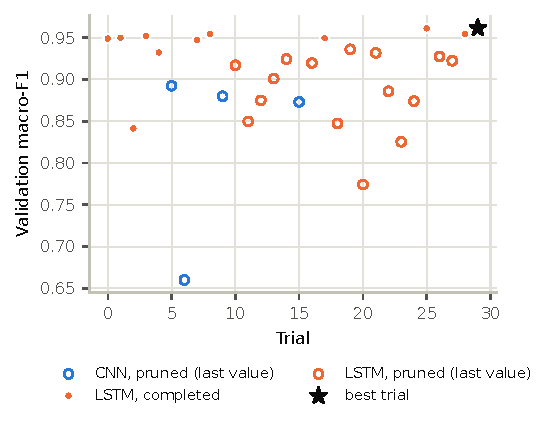
\includegraphics[width=0.55\linewidth]{../../figures/phase4/p4_search.pdf}
\caption{Search: best validation macro-F1 of each trial; for pruned trials the last value before pruning.}\label{fig:search}
\end{figure}

% =====================================================================
\section{Final models}\label{sec:final}

The chosen configuration was trained with five seeds for at most 40 epochs, stopping after six epochs without improvement of the validation macro-F1 (Figure~\ref{fig:curves}). Each training took 2 to 3 minutes. The best validation macro-F1 was 0.9616, 0.9580, 0.9629, 0.9625 and 0.9513 for seeds 0 to 4, reached at epoch 2 to 5. The training loss keeps falling while the validation loss stays between 0.14 and 0.31 from the second epoch on, and the validation macro-F1 moves by several hundredths from one epoch to the next (0.82 to 0.96 over all epochs of the five seeds): the network fits the training runs quickly, and which epoch is kept depends on the validation set. This is why the test runs, which played no part in that choice, are the only fair measure. The protocol deploys the seed with the highest validation macro-F1, seed 2.

\begin{figure}[h]
\centering
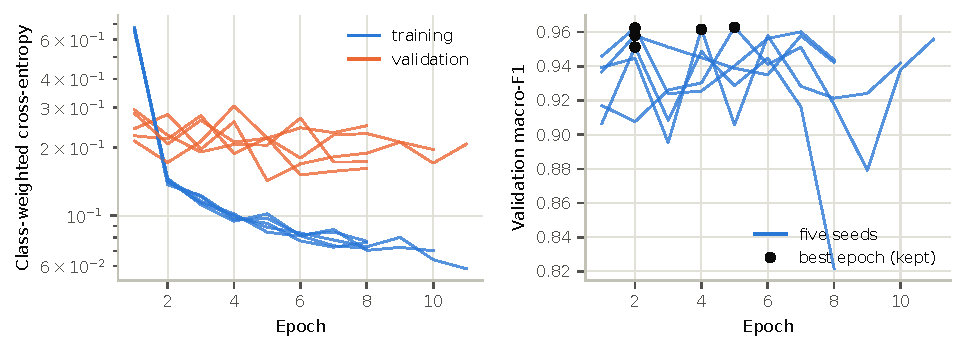
\includegraphics[width=\linewidth]{../../figures/phase4/p4_learning_curves.pdf}
\caption{Learning curves of the five seeds of the chosen configuration (training and validation runs).}\label{fig:curves}
\end{figure}

Trained on a quarter and on half of the training runs (66 and 132 runs, the first in the order repetition, cable, fault, with the fault free runs in proportion; seeds 0--2), the same configuration reached a validation macro-F1 of 0.744 to 0.820 and of 0.855 to 0.909, against 0.958 to 0.963 with all 264 runs (Figure~\ref{fig:size}). The curve has not flattened: more training runs would very likely give a better classifier, which matters when it is compared with the IMM.

\begin{figure}[h]
\centering
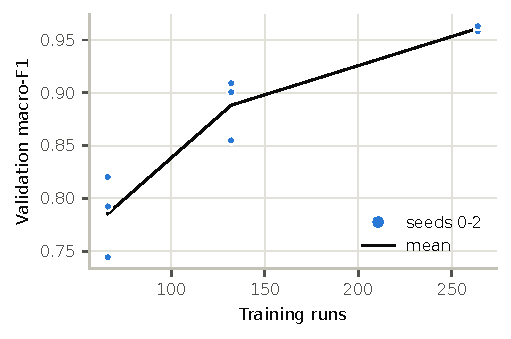
\includegraphics[width=0.5\linewidth]{../../figures/phase4/p4_size_curve.pdf}
\caption{Validation macro-F1 against the number of training runs.}\label{fig:size}
\end{figure}

% =====================================================================
\section{Declaration thresholds}\label{sec:thr}

The controller declares a fault when the same fault mode is the most probable, with probability at least $\mu_{\mathrm{iso}}$, in $N_c$ consecutive estimator cycles (methods, Sec.~7.3). The rule is applied to the classifier's probabilities on every validation run for the 48 pairs of the protocol (\path{cdpr_ft/learning/declare.py}; a test checks that it gives the same results as the Phase~3 threshold study), and the pair is chosen by the rule of the protocol: fewest runs with a false alarm, then most faults declared with the correct mode, then the smallest median delay of the break declarations, then the larger $\mu_{\mathrm{iso}}$ and $N_c$. When a pair has no false alarm and isolates every fault, this is the rule that chose the IMM's thresholds in Phase~3, and on the stored Phase~3 table it chooses the same pair (a test checks this).

For the deployed model the rule chose $\mu_{\mathrm{iso}}=0.99$ and $N_c=4$ (Figure~\ref{fig:thr}). On the validation runs this gives no false alarm, all 16 breaks and all 32 losses of effectiveness declared correctly (median delays 32 and 38~ms) and 26 of the 32 biases (median 102~ms). No pair without false alarms isolates every bias: the best of the five seeds reaches 31 of 32. For the other seeds the rule chose $(0.99, 8)$, $(0.95, 8)$, $(0.95, 8)$ and $(0.99, 1)$, with 79, 74, 77 and 77 correct declarations out of 80.

\begin{figure}[h]
\centering
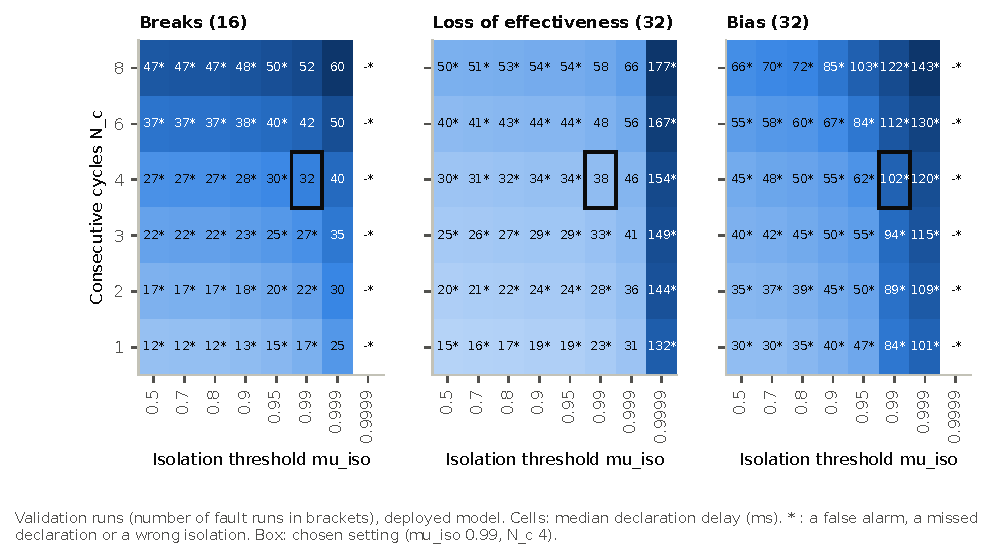
\includegraphics[width=\linewidth]{../../figures/phase4/p4_thresholds.pdf}
\caption{Threshold study of the deployed model on the validation runs.}\label{fig:thr}
\end{figure}

% =====================================================================
\section{Frozen classifier}\label{sec:freeze}

\path{configs/classifier_phase4.yaml} records the hyperparameters, the five models with their file hashes, the deployed model (seed 2) with its thresholds, and the hashes of the protocol, the dataset, the code of the inputs and of the networks, and the digest of the controller code, which is still that of the Phase~3 freeze (\texttt{fe7722d2d710c537}): Phase~4 added files to the package and changed none. The test script refuses to run if any of these has changed since the freeze, and refuses to overwrite its result unless asked to repeat it. The deployed network has 57\,425 parameters and takes 0.9~ms per window on this machine (median; 1.5~ms at the 99th percentile), well inside the 5~ms period of the estimator.

% =====================================================================
\section{Test evaluation}\label{sec:test}

The test runs were evaluated once, on 27 October 2026, after the frozen file of Section~\ref{sec:freeze} had been written. The IMM is evaluated on the same runs and the same estimator cycles, with its frozen thresholds ($\mu_{\mathrm{iso}}=0.9999$, $N_c=2$, fixed in Phase~3 on calibration runs). Window results count every cycle from 2~s to the end of a run; run results apply the declaration rule; intervals are 95\% bootstrap intervals over runs \citep{efron1993bootstrap} (2000 resamples, the same resample for both methods, so that the difference has its own interval).

\begin{table}[h]
\centering\small
\caption{Single test evaluation. Deployed classifier (seed 2, $\mu_{\mathrm{iso}}=0.99$, $N_c=4$) and IMM (frozen, $\mu_{\mathrm{iso}}=0.9999$, $N_c=2$) on the same runs, 88 per path, 80 of them with a fault. A fault run with a false alarm before its onset counts as a false alarm, not as a declaration of its fault (25 of the T2 fault runs for the classifier). Delays are those of the correct declarations, from the onset. Brackets: 95\% bootstrap intervals over runs.}\label{tab:test}
\begin{adjustbox}{max width=\linewidth}\begin{tabular}{@{}lllll@{}}
\toprule
 & \multicolumn{2}{c}{T1, test runs} & \multicolumn{2}{c}{T2, path not seen in training} \\
\cmidrule(lr){2-3}\cmidrule(lr){4-5}
 & Classifier & IMM & Classifier & IMM \\
\midrule
Cycles labelled correctly & 0.980 & 0.996 & 0.591 & 0.996 \\
Macro-F1 over cycles & 0.933 & 0.991 & 0.700 & 0.990 \\
Runs with a false alarm, of 88 (\%) [interval, \%] & 1 (1\%) [0, 3] & 0 (0\%) [0, 0] & 31 (35\%) [26, 45] & 0 (0\%) [0, 0] \\
Faults declared correctly, of 80 (\%) [interval, \%] & 73 (91\%) [85, 97] & 80 (100\%) [100, 100] & 45 (56\%) [45, 67] & 80 (100\%) [100, 100] \\
Faults missed / declared as another mode & 1 / 5 & 0 / 0 & 0 / 10 & 0 / 0 \\
Breaks declared correctly & 16 of 16 & 16 of 16 & 8 of 16 & 16 of 16 \\
\quad delay: median [interval]; max (ms) & 31 [30, 34.5]; 39 & 15 [15, 16]; 18 & 32 [28, 37]; 38 & 17 [16, 18]; 18 \\
Losses of effectiveness declared correctly & 31 of 32 & 32 of 32 & 22 of 32 & 32 of 32 \\
\quad delay (ms) & 38 [37, 40]; 50 & 23 [22, 25]; 35 & 41.5 [39, 51]; 87 & 22 [19, 23]; 32 \\
Biases declared correctly & 26 of 32 & 32 of 32 & 15 of 32 & 32 of 32 \\
\quad delay (ms) & 106 [72.5, 120]; 415 & 43 [33, 58]; 98 & 93 [61, 124]; 262 & 39.5 [35, 48]; 69 \\
\bottomrule
\end{tabular}\end{adjustbox}
\end{table}

\begin{table}[h]
\centering\small
\caption{Paired differences, classifier minus IMM: 95\% bootstrap intervals over runs (same resample for both methods).}\label{tab:diff}
\begin{tabular}{@{}lll@{}}
\toprule
 & T1, test runs & T2 \\
\midrule
Faults declared correctly (percentage points) & [$-15.4$, $-2.8$] & [$-55.0$, $-33.3$] \\
Runs with a false alarm (percentage points) & [0.0, 3.4] & [26.1, 45.5] \\
Median delay, breaks (ms) & [14, 19.5] & [11, 20.5] \\
Median delay, losses of effectiveness (ms) & [13.5, 17] & [16.5, 29] \\
Median delay, biases (ms) & [27, 85] & [20, 85] \\
\bottomrule
\end{tabular}
\end{table}

\paragraph{On the path it was trained on (T1).} The deployed classifier labels 98.0\% of the cycles correctly (macro-F1 0.933), declares all 16 breaks correctly and 31 of the 32 losses of effectiveness, the remaining one being a false alarm before its onset, and 26 of the 32 biases; it misses one bias and isolates five as an actuator fault of the neighbouring lower winch (cable 5 as 6 twice, 6 as 5, 7 as 8 twice). Its declarations take about twice as long as those of the IMM: 31 against 15~ms for the breaks, 38 against 23~ms for the losses of effectiveness and 106 against 43~ms for the biases (medians), and the paired intervals of the differences exclude zero for all three (Table~\ref{tab:diff}); so does the interval of the difference in correct declarations, $-15.4$ to $-2.8$ percentage points. The IMM declares all 80 faults correctly and has no false alarm. The five seeds give a macro-F1 of $0.942\pm0.009$ and $94.5\pm3.6\%$ correct declarations (mean $\pm$ standard deviation). The deployed seed, chosen by its validation macro-F1, is not the best of the five on the test runs: its test macro-F1 is the lowest (0.933, against 0.935 to 0.953), and seeds 0 and 1 declare 78 of the 80 faults correctly. Validation scores between 0.951 and 0.963, on 88 validation runs, do not rank the five models reliably, which is worth a sentence in the paper.

\paragraph{On the held out path (T2).} The classifier does not carry over to the helix. It labels only 54\% of the healthy cycles as healthy, taking 23\% of them for an actuator fault of winch~5 and 14\% for one of winch~7; 31 of the 88 runs have a false alarm, among them 6 of the 8 fault free runs, and 45 of the 80 faults are declared correctly. Breaks are still recognised when they come: the classifier labels 96 to 99\% of the break cycles correctly, and the eight break runs not counted as correct are runs with a false alarm before the onset. It is therefore the healthy motion along the climbing path, never seen in training, that the network maps to actuator faults of the lower winches. The five seeds agree ($0.717\pm0.031$ macro-F1, $22.6\pm7.8$ runs with a false alarm). The IMM, which uses a model of the robot rather than examples of its motion, keeps its performance on T2: no false alarm, all 80 faults declared correctly, median delays of 17, 22 and 39.5~ms.

\begin{figure}[h]
\centering
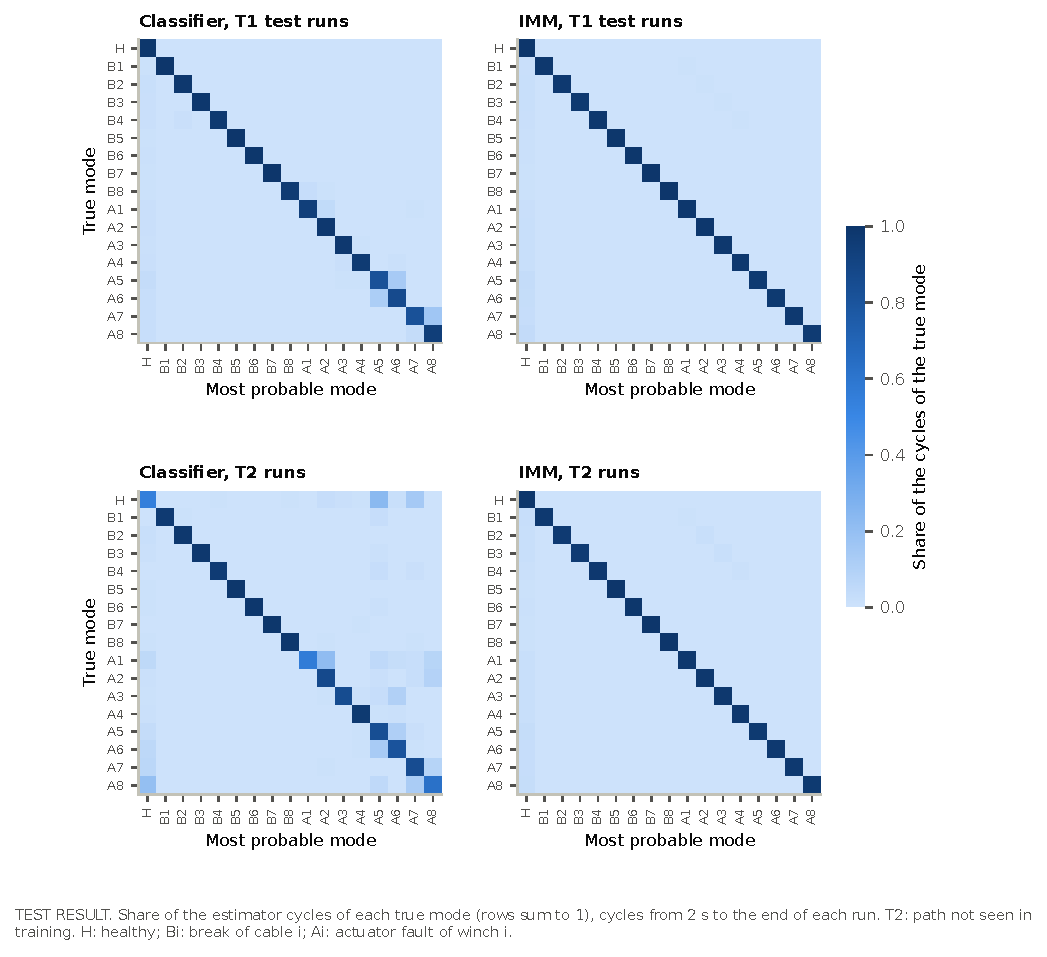
\includegraphics[width=\linewidth]{../../figures/phase4/p4_test_confusion.pdf}
\caption{Test result: confusion matrices per estimator cycle, deployed classifier and IMM, on the T1 test runs and on the T2 runs.}\label{fig:confusion}
\end{figure}

\begin{figure}[h]
\centering
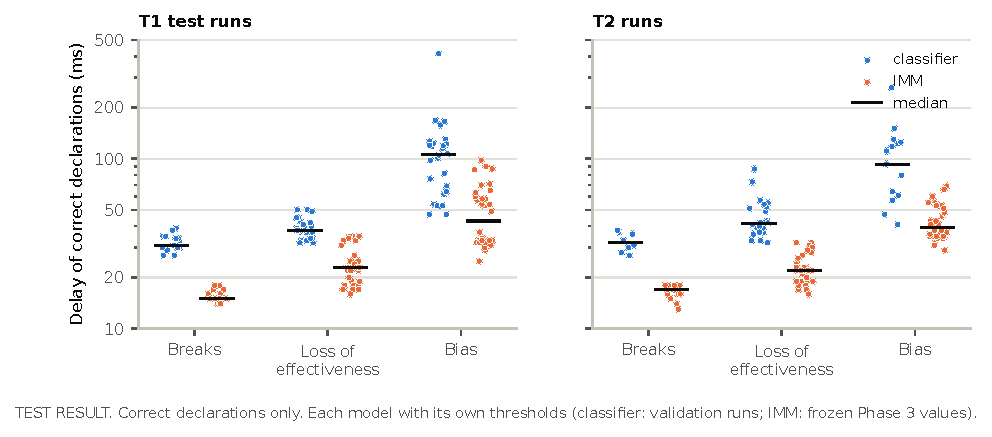
\includegraphics[width=\linewidth]{../../figures/phase4/p4_test_delays.pdf}
\caption{Test result: delays of the correct declarations by fault type.}\label{fig:delays}
\end{figure}

\paragraph{What this says, and what it does not.} On the path it was trained on, a recurrent network of 57\,425 parameters, trained on 264 runs, detects and isolates the faults of this robot, but later than the IMM and with less certainty about biases; on a path it has not seen it raises false alarms in a third of the runs. The size curve has not flattened, the search tried few convolutional networks, and the network was trained on one path only, by design of the specification. A classifier trained on more runs and on several paths would do better; how much better is not known from this study, and B3 is one well documented learned baseline, not the best a learned detector can do.

% =====================================================================
\section{Changes to the protocol}\label{sec:amend}

The protocol was written before the first Phase~4 run and was changed twice, both times before the dataset was built and before any search trial; the protocol file records both with the hash of the version they replaced.
\begin{enumerate}
\item \emph{Compression of the inputs.} While the first runs were simulated it became clear from the calibration records that the length residual of a broken cable reaches metres, while the residuals that reveal an actuator fault are millimetres. A linear standardisation would have squeezed the latter, so the signed logarithm was added in front of it (Section~\ref{sec:inputs}).
\item \emph{Compute budget.} A timing check on this two-core machine, one thread, batches of 256 windows, gave 0.04~s per training step for a convolutional network of three layers of 32 channels with kernel 5 over 40 cycles, and 0.53~s for an LSTM of two layers of 128 units over 80 cycles. The largest configurations of the first search space would have taken hours per epoch and the search days. The space was narrowed (at most 64 channels, kernels 3 and 5, at most 64 units), the epochs of a trial were limited to 20 with patience 4 and those of the final training to 40 with patience 6, and the fault windows of the training split are taken every second cycle. The timing check trained two small models for one and two epochs on the first 14 finished training and validation runs, and a check of determinism trained one model for one epoch twice on the full training split; none of their scores was used for any choice.
\end{enumerate}
The runs themselves were simulated in three invocations of the script (the container of the machine was restarted once); every run is determined by its seed, and Section~\ref{sec:repro} shows that runs regenerated afterwards are identical to the stored ones.

% =====================================================================
\section{Reproduction}\label{sec:repro}

Every run is fixed by its seed: the plant parameters, the noise, the fault and its onset are drawn from generators seeded from it, and the simulation itself is deterministic. Four runs simulated again after the dataset had been built (runs 5 and 300 of the training split, the fault free validation run 430 and the T2 run 500) gave records, IMM probabilities and metrics identical to the stored ones (1\,386\,951 array values). The networks are trained on the CPU with deterministic algorithms and a fixed number of threads (two); training the same model twice gave identical weights.

Every step after the simulation of the runs was then repeated with \texttt{reproduce.py phase4} on the same machine, in the working copy of the repository, and each output was compared with the stored file (Table~\ref{tab:repro}). Every compared value agreed to the last bit; the five model files and the frozen file are even identical byte for byte. The search and the final training are therefore exactly reproducible on this platform, and the test result of Section~\ref{sec:test} is what the stored code, data and models give. On another processor the kernels of torch may round differently, and a search or a training may then take a slightly different path; \path{REPRODUCE.md} describes this and how the test step alone checks the evaluation from the stored models.

\begin{table}[h]
\centering\small
\caption{Repetition of the Phase 4 steps (two cores; the search and the training shared the machine with other work at times).}\label{tab:repro}
\begin{tabular}{@{}lrl@{}}
\toprule
Step & Time [min] & Outcome \\
\midrule
Runs (\path{phase4_generate.py}) & 123 & original generation; four runs simulated again: identical \\
Dataset & 6.2 & identical, 18\,741\,219 values and the run list \\
Search & 55.9 & identical, 30 trials \\
Training & 17.2 & identical histories, size curve and five models (57\,483 values each) \\
Thresholds & 0.3 & identical \\
Freeze & 0.0 & identical \\
Test & 0.7 & identical, 7880 values \\
\bottomrule
\end{tabular}
\end{table}

The automated tests of the repository (51, of which 7 are new in this phase) pass. The new ones check that the input stream hands the network the same tension averages and lengths, cycle by cycle, that the diagnosis hands the IMM; that the declaration rule gives the results of the Phase~3 threshold study on the stored Phase~3 probabilities and chooses the same thresholds; the shapes of the networks and that the convolutional network sees the newest cycle; and that training is deterministic.

% =====================================================================
\section{Carried into Phase 5}\label{sec:next}

\paragraph{How B3 enters the controller.} The specification puts the learned classifier in place of the IMM. The controller uses the IMM for two different things: its mode probabilities decide the declaration and, in the proposed controller, weight the fault scenarios of the MPC before a declaration; its filters give the state of the platform, and after a declaration the state and the deficit of the declared mode. The classifier gives only the first. The proposal for Phase~5 is therefore that B3 replaces the mode probabilities, with its own thresholds ($\mu_{\mathrm{iso}}=0.99$, $N_c=4$), while the filters keep running as the state estimator. B3 then differs from the proposed controller in the diagnosis only, which is the comparison the baseline is meant to make. The estimator cycle then costs the IMM's 2.3~ms (mean, Phase~3) plus the classifier's 0.9~ms.

\paragraph{Training path.} The classifier of this phase was trained on the circle T1 only, as the specification asks, so that the held out helix measures generalisation; on T2 it raises false alarms in about a third of the runs. The Phase~5 campaign runs both paths. Used as it is, B3 would lose on T2 because it never saw that path, which the design of its training explains in advance. A second model, with the same hyperparameters and the same rules for the thresholds, trained on runs of both paths (new seeds in the Phase~4 range, about 1.5~h of runs and under 1~h of training on this machine) would be the fairer baseline for the campaign, with the model of this phase kept as the generalisation result. This is a decision for the authors before Phase~5 starts.



\bibliographystyle{plainnat}
\bibliography{phase4}
\end{document}
